\section{\TheName{} System Model}\label{sec:3}
In this section, we first formulate the research problem of our study, then we describe the \TheName{} framework to solve the formulated problem.

\subsection{Problem Formulations}
According to our research assumptions, we make two definitions and introduce several preliminary studies that we use. Further, we formulate our research problem based on these definitions and preliminaries.

\textbf{\em Definition I.} \emph{Diagnosis-frequency Vector and Non-negative Noise Vector --- } Given EHR data of $m$ patients (both with and without the targeted disease), we can extract $m$ diagnosis-frequency vectors $X_0,X_1\dots X_{m-1}$. Each vector (e.g., $X_i=<1,0,\dots,3>$) consists of two parts: (1) $\hat{X}_1$, the vector of true diagnosis frequencies (not diagnosis record frequencies), and (2) $E_i$, the non-negative noise vector:
\begin{equation}
X_i=\hat{X}_1+E_i
\end{equation}

\textbf{\em Preliminary I. } \emph{Generalized Two-class LDA and Covariance Matrices --- } 
In typical implementations of an LDA classifier~\cite{ziegel2003modern}, given $m$ training samples as well as the labels $(X_0,l_0)\dots (X_{m-1},l_{m-1})$, where $l_i\in\{-1,+1\}$ indicates whether the patient $i$ has been diagnosed with the target disease (i.e., positive sample or negative sample), a two-class LDA model first sorts each sample into two groups according to the label, and estimates covariance matrix/mean vector of the two classes, ($\Sigma_{+}$, $\mu_+$) and ($\Sigma_{-}$,$\mu_-$) using the positive samples and negative samples, respectively.  
Then, generalized two-class LDA determines whether a new patient ($X'$) would develop to the targeted disease, using
%
\begin{equation}
\begin{aligned}
&(X'-\mu_-)^T\Sigma_{-}^{-1}(X'-\mu_-)+ln|\Sigma_-|-\\
&(X'-\mu_+)^T\Sigma_{+}^{-1}(X'-\mu_+)-ln|\Sigma_+|<T,
\end{aligned}
\label{eq:glda}
\end{equation}
%
where $T$ is an optimal threshold based on the training samples. However, as illustrated in Observation 2,  when positive sample size is relatively small (e.g., for a rare disease in the database),  $Rank(\Sigma_+)<p$,  $\Sigma_{+}$ is singular and $\Sigma_{+}^{-1}$  does not exist. In this case, Equation~\ref{eq:glda} might not work.

Note that hereafter, we refer to both $\Sigma_{+}$ and $\Sigma_{-}$ as \emph{covariance matrices} because they are both considered equal in our problem formulation and solution design.


\textbf{\em Definition II.} \emph{Sample Diagnosis-to-Diagnosis Covariance Matrix Estimation and Disturbance of Non-negative Noise --- } With the above settings in mind, we further define $\Sigma$ as the sample diagnosis-to-diagnosis covariance matrix based on noisy data, $\hat{\Sigma}$, as the sample covariance matrix based on ``noisy-free'' vectors, and  $\Delta=\Sigma-\hat{\Sigma}$ as the disturbance of non-negative noise to covariance estimation.
%
\begin{equation}
\begin{aligned}
\Sigma&=\frac{1}{n}\sum_{i=0}^{n-1} X_iX_i^T
=\frac{1}{n}\sum_{i=0}^{n-1} (\hat{X}_i+E_i)(\hat{X}_i+E_i)^T\\
&=\hat{\Sigma}+\Delta
\end{aligned}
\label{eq:sample-cov}
\end{equation}
As the sample covariance matrix estimation shown in~\ref{eq:sample-cov}, the disturbance should be:
%
$$\Delta=\frac{1}{n}\sum_{i=0}^{n-1}(2\hat{X}_iE_i^T+E_iE_i^T).$$ 
%
According to our definition, $\hat{X}_i$ and $E_i$ are both non-negative matrices. 
From this, we find that $\Delta=\Sigma-\hat{\Sigma}\geq \textbf{0}$ is a non-negative matrix and $||\Sigma||\geq ||\hat{\Sigma}||$. 
Thus, we can conclude that $\hat{\Sigma}$ might be a sparse estimation of $\Sigma$. 

\textbf{\em Preliminary II. } \emph{Minimax decision risk estimation of the covariance matrix in HDLSS settings --- } Previous work~\cite{cai2012minimax,xue2012positive} showed that it is possible to achieve \emph{minimax risk} covariance matrix estimation from a few samples, using the \emph{minimal $\ell^1$-normal estimation} of the original sample covariance matrix. 
In this case, in terms of lowering variance of LDA, we can assume that the optimal~\cite{cai2012minimax} covariance matrix $\tilde{\Sigma}$ should be a $\ell^1$-penalized sparse estimation of $\hat{\Sigma}$.

\textbf{Problem Formulation. } According to the definitions and preliminaries above, this paper considers the problem of finding the positive-definite sparse estimation of $\hat{\Sigma}$---the noise-free diagnosis-to-diagnosis covariance matrices, to improve the performance of LDA for early detection of disease. 
We define our research problem that in the following way: given $n$ diagnosis-frequency vectors $X_0,X_1\dots X_{n-1}$,  our problem is to estimate $\tilde{\Sigma}$:
\begin{equation}
\begin{aligned}
\text{min. }|\tilde{\Sigma}|_1 \text{ s.t. }||\tilde{\Sigma}-\hat{\Sigma}||_F^2\leq \epsilon\text{ and }\tilde{\Sigma}\in {\bf }I^+
\end{aligned}
\label{eq:problem}
\end{equation}
where ${\bf }I^+$ refers to the overall set of positive semidefinite matrices. Note that $\hat{\Sigma}$ is not foreknown due to the unknown data noise. 

Intuitively, it is possible to solve the formulated problem through sparsifying and regularizing the sample diagnosis-to-diagnosis covariance matrix $\Sigma$ that is positive semidefinite and non-singular. 


\begin{figure}
\begin{center}
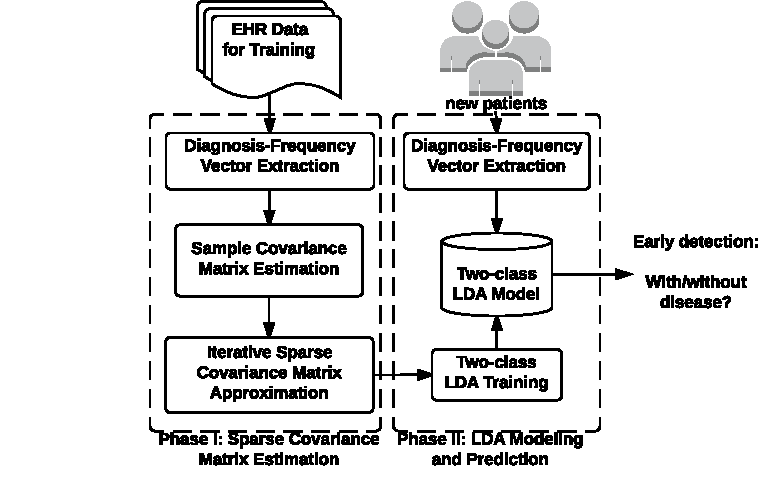
\includegraphics[width=0.48\textwidth]{./img/daehr.pdf}
\end{center}
\caption{\TheName\ Framework}
\end{figure}


\subsection{\TheName\ Framework}
In this section, we introduce the framework design of \TheName{}. 
\TheName{} consists of two phases.  
First, we use the EHR data for training to estimate the covariance matrices used in LDA with respect to our problem formulation. 
Next, we adopt LDA with newly estimated parameters to predict whether the new patient will develop the targeted disease.

\emph{Phase I: Sparse Covariance Matrix Estimation --- } Given the patients' EHR data as a training set, this phase estimates the sparse covariance matrices for two classes of patients with following two steps:
\begin{enumerate}
    \item \textbf{Diagnosis-frequency Vector Extraction and Sample Covariance Matrix Estimation --- } \TheName{} first converts each patient's EHR data to a diagnosis-frequency vector and combines it with his/her label (indicating whether the patient has been diagnosed with the targeted disease). Specifically, we acquire $(X_0,l_0)\dots (X_{m-1},l_{m-1})$, where $l_i\in\{-1,+1\}$ is the label of the $i^{th}$ patient. With the vectors corresponding to each of the two classes, \TheName{} then estimates the sample covariance matrices for the two classes $\Sigma_+$ and $\Sigma_-$ using Equation~\ref{eq:sample-cov}.

    \item \textbf{Iterative Sparse Covariance Matrix Approximation --- } Given sample covariance matrices $\Sigma_+$ and $\Sigma_-$, \TheName{} estimates the positive-definite $\ell^1$-penalized estimation of both $\Sigma_+$ and $\Sigma_-$ using a unified iterative approximation process, where \TheName{} treats $\Sigma_+$ and $\Sigma_-$ equally. 
    As shown in Algorithm~\ref{alg:iap}, given an input sample covariance matrix $\Sigma_0=\Sigma_+$ or $\Sigma_-$, the process iteratively approximates to the positive definite $\ell^1$-penalized estimation of $\Sigma_0$ through alternating between two algorithms---\emph{$\ell^1$-penalized Sparse Matrix Estimation} and \emph{Nearest Positive Semidefinite Matrix Approximation} in each iteration. In Algorithm~\ref{alg:iap}, $\Delta'=\frac{||\Sigma_{t+1}-\Sigma_{t}||_\infty}{||\Sigma_{t}||_\infty}$ and $tol$ is a threshold characterizing the tolerance of convergence. 
    Specifically, in each (i.e., the $t^{th}$, $t\geq 0$) iteration, the process obtains an improved result $\Sigma_{t+1}$ using the previous result $\Sigma_{t}$. 
    With the result improved each iteration, the algorithm stops only when the predefined convergence is achieved ($\Delta''< tol$) or after iterating $maxit'$ times (i.e., $t>maxit'$).


\end{enumerate}
Note that the covariance matrices for the two classes of patients are estimated in this phase through a unified process.
We denote the new covariance matrices as $\Sigma_+^*$ and $\Sigma_-^*$ for the positive and negative classes, respectively.

\begin{algorithm}
\caption{Iterative Approximation Process for Sparse Covariance Matrix Estimation}
\label{alg:iap}
\KwData{$\Sigma_{0}$ --- the sample covariance matrix i.e., $\Sigma_+$ or $\Sigma_-$}
\KwResult{${\Sigma_{t+1}}$ --- the positive definite $\ell^1$-penalized estimation of $\Sigma_0$}
\Begin{
\While{ $\Delta' \geq tol, \text{ or }0\leq t \leq maxit'$  }{
	$\Sigma_{t+\frac{1}{2}}\gets \ell^1$-penalized sparse estimation of $\Sigma_t$
    $\Sigma_{t+1}\gets $ the nearest positive semidefinite approximation to  $\Sigma_{t+\frac{1}{2}}$
}
\Return{$\Sigma_{t+1}$}
}
\end{algorithm}


\emph{Phase II: LDA Modelling and Prediction --- } Given the two estimated matrices $\Sigma_+$ and $\Sigma_-$ as well as the training samples, this phase first trains the optimal model for LDA prediction. 
Then, it uses the LDA model for new patient prediction. 
This phase consists of following two steps:
\begin{enumerate}
    \item \textbf{LDA Model Training --- } Given the two estimated covariance matrices $\Sigma_+^*$ and $\Sigma_-^*$ as well as training samples $(X_0,l_0)\dots (X_{m-1},l_{m-1})$, \TheName{} searches for the optimal threshold $T^*$ that can maximally classify the two classes of samples using Equation~\ref{eq:glda}. 
        In this case, \TheName{} uses a LDA model as $(\Sigma_+^*,\mu_+,\Sigma_-^*,\mu_-,T^*)$.
    \item \textbf{LDA-based new Patient Prediction --- } Given a new patient's EHR data, \TheName{} first converts her data to a diagnosis-frequency vector (e.g., $X'$). 
        Combined with the LDA model described as $(\Sigma_+^*,\mu_+,\Sigma_-^*,\mu_-,T^*)$, \TheName{} predicts whether the patient will develop the targeted disease using the criterion in Equation~\ref{eq:glda}.
\end{enumerate}
%

After the above two phases terminate, \TheName{} will have (1) learned a LDA model with advanced covariance matrix estimation, and (2)  adopted the LDA model to enable the early detection of targeted disease. 
Though the architecture of the framework is discussed here, the design of the aforementioned \emph{$\ell^1$-penalized Sparse Matrix Estimation} and \emph{Nearest Positive Semi-Definite Matrix Approximation} algorithms are discussed in following sections.

